\thispagestyle{empty}
\graphicspath{{1axioms/asy/}}

\title{Math 161 - Notes}
\author{Neil Donaldson}
\date{Spring 2024}
\maketitle


\section{Geometry and the Axiomatic Method}\label{chap:axioms}

\subsection{The Early Origins of Geometry: Thales and Pythagoras}\label{sec:thales}


We begin with a condensed overview of geometric history. The word \emph{geometry} comes from the ancient Greek \emph{geo} (Earth), and \emph{metros} (measure). Measurement (of distance, area, height, angle) had obvious practical benefits with regard to construction, taxation, commerce and navigation. Astronomy provided a related cultural driver of ancient geometry.

\begin{description}
	\item[Ancient times] (pre-500\,\BC) Egypt, Mesopotamia, China, India: basic rules for measuring lengths, areas and volumes of simple shapes. Applications: surveying, tax collection, construction, religious practice, astronomy, navigation. Typically worked examples without general formulæ/abstraction.
	
	\item[Ancient Greece] (from c.\,600\,\BC) Philosophers such as Thales and Pythagoras began the process of \emph{abstraction.} General statements (theorems) formulated and proofs attempted. Concurrent development of early scientific reasoning.
	
	\item[Euclid of Alexandria] (c.\,300\,\BC) Collected and expanded earlier work, especially that of the Pytha\-goreans. His compendium the \emph{Elements} is one of the most important books in Western history and remained a standard school textbook in to the 1900's. The \emph{Elements} is an early exemplar of the axiomatic method at the heart of modern mathematics.
	
	\item[Later Greek Geometry] Archimedes' (c.\,270--212\,\BC) work on area and volume included techniques similar to those of modern calculus. %Apollonius studies conics (ellipses, parabolæ and hyperbolæ).
	Ptolemy (c.\,\AD\,100--170) writes the \emph{Almagest}, a treatise on astronomy which covers the foundations of trigonometry.
	
	\item[Post-Greek Geometry] During the European Dark Ages, geometric understanding was developed and enhanced by Indian and Islamic mathematicians who particularly developed trigonometry and algebra.
	
	\item[Analytic Geometry] In mid 1600's France, Descartes and Fermat melded algebra with geometry with the advent of co-ordinate systems (axes).
 	
	\item[Modern Development] Non-Euclidean geometries help provide the mathematical foundation for Einstein's relativity and the study of curvature. Following Klein (1872), modern geometry is highly dependent on group theory.
\end{description}



\boldinline{Thales of Miletus (c.\,624--546\,\BC)}

Thales was an olive trader from Miletus, a city-state on the west coast of modern Turkey. Through trading and travelling, he absorbed mathematical ideas from nearby cultures including Egypt and Mesopotamia. Here are five results partly attributable to Thales.

\begin{enumerate}\itemsep0pt
  \item A circle is bisected by a diameter.
  \item The base angles of an isosceles triangle are equal.
  \item The pairs of angles formed by two intersecting lines are equal.
  \item Two triangles are congruent if they have two angles and the included side equal.
  \item An angle inscribed in a semicircle is a right angle.
\end{enumerate}
The last is still known as \emph{Thales' Theorem.} Thales' arguments were not rigorous by modern standards. His real innovation was to state \emph{abstract, general principles}: \emph{any} circle is bisected by \emph{any} of its diameters. The Greek word $\theta\varepsilon\omega\rho\varepsilon\omega$ (\emph{theoreo}), from which we get \emph{theorem,} has several meanings: `to look at,' `speculate,' or `consider.' Thales' results were supposed to be clear just by looking at a picture.
\begin{center}
	\includegraphics[scale=0.9]{thales-1}
	\qquad\qquad
	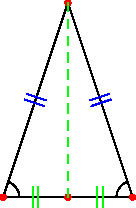
\includegraphics[scale=0.9]{thales-2}
	\qquad\qquad
	\includegraphics[scale=0.9]{thales-5}\label{thm:thales}
\end{center}
The pictures show Thales' Theorems 1, 2 and 5. Arguments for Theorems 1 and 2 could be as simple as `fold.' Theorem 5 follows from the observation that the \textcolor{Green}{radius} of the circle splits the large triangle into two isosceles triangles: Theorem 2 says that these have equal base angles (labelled), now check that $\alpha+\beta$ is half the angles in a triangle, namely a right-angle.


\boldinline{Pythagoras of Samos (570–-495\,\BC)}

Pythagoras grew up on Samos, an island in the Aegean Sea not far from Miletus. He also travelled widely, eventually settling in Croton, southern Italy, around 530\,\BC{} where he founded a philosophical school devoted to the study of number, music and geometry. It has been claimed that the Pythagoreans first classified the regular (Platonic) solids and developed the musical relationship between the length of a vibrating string and its pitch. While it is difficult to verify such assertions, the Pythagorean obsession with number and the `music of the universe' certainly inspired later mathematicians and philosophers---particularly Euclid, Plato and Aristotle---who believed they were refining and clarifying this earlier work.
\smallbreak

Of course, Pythagoras is best known for the result that bears his name.

\begin{thm}{Pythagoras}{}
	The square on the hypotenuse of a right triangle equals the sum of the squares on the remaining sides.
\end{thm}

Two important clarifications are needed for modern readers.
\begin{enumerate}\itemsep0pt
  \item By \emph{square,} the Greeks meant an honest square! There is no algebra, no numerical lengths, and the equation $a^2+b^2=c^2$ won't be seen for another 2000 years.
  \item The word \emph{equals} means \emph{equal area,} though without a numerical concept of such. The Greeks meant that the large square can be subdivided into pieces which may be rearranged to produce the two squares on the remaining sides.
\end{enumerate}

\goodbreak

The result suddenly seems less easy! The pictures below provide a simple visualization.

\begin{center}
	\includegraphics[width=0.3\linewidth]{pythag}
	\qquad\qquad\qquad\qquad
	\includegraphics[width=0.3\linewidth]{pythag2}
	\medbreak
	A simple proof of Pythagoras' Theorem
\end{center}
The problem with this `proof' is that it relies on \emph{subtracting} the areas of the four congruent triangles from a very large square, whereas the Greeks idea of area was essentially \emph{additive.} Book I of Euclid's \emph{Elements} seems to have been structured precisely to correct this and provide a rigorous constructive proof. Indeed it is possible (though very ugly!) to apply the 47 results leading up to and including his proof of Pythagoras, in such as way as to explicitly subdivide the hypotenuse square and rearrange it into the two smaller squares as required.
\smallbreak


Much has been written about Pythagoras' Theorem, including many, many proofs.\footnote{Including a \href{https://www.maa.org/press/periodicals/convergence/mathematical-treasure-james-a-garfields-proof-of-the-pythagorean-theorem}{proof} by former US President James Garfield. Would that current presidents were so learned\ldots} It is often claimed that Pythagoras himself first proved the result, but this is generally considered incorrect---the `proof' most often attributed to the Pythagoreans is based on contradictory ideas about numbers which were debunked by the time of Aristotle. Moreover, other cultures, particularly ancient China,\footnote{In China, Pythagoras' Theorem is known as the \emph{gou gu,} which refers to the two non-hypotenuse sides of the triangle.} are known to have used the result, at least in example form, several hundred years before Pythagoras. Regardless, an argument over attribution is fruitless without first agreeing on what constitutes a proof. This means that we need to spend some time considering Axiomatic Systems\ldots 


\begin{exercises}{}{}
	\exstart Let the side-lengths of the above triangles be $a,b,c$. Can you rephrase the proof algebraically?
	\begin{enumerate}\setcounter{enumi}{1}
		\item A theorem of Euclid states:
		\begin{quote}
			The square on the parts equals the sum of the squares on each part plus twice the rectangle on the parts
		\end{quote}
		By referencing the above picture, state Euclid's result using modern \emph{algebra.}\par
		(\emph{Hint: let $a$ and $b$ be the `parts'\ldots})
	\end{enumerate}
\end{exercises}

\clearpage



\subsection{Axiomatic Systems}

%A primary motivation for Euclid's writing of the first book of the \emph{Elements} was to rigorously prove Pythagoras' Theorem. In so doing, he essentially invented the modern axiomatic method. %Before considering Euclid's approach, we describe the revolutionary structure Euclid followed, that of a \emph{deductive} or \emph{axiomatic system.}

Arguably the most revolutionary aspect of the Euclid's \emph{Elements} was its axiomatic presentation.

\begin{defn}{}{}
	An \emph{axiomatic system} comprises four types of object.\vspace{-5pt}
	\begin{enumerate}\itemsep0pt
	  \item \emph{Undefined terms}: Concepts accepted without definition/explanation. %In basic geometry these would include \emph{line} and \emph{point.}
	  \item \emph{Axioms}: Logical statements regarding the undefined terms which are accepted without proof.
	  \item \emph{Defined terms}: Concepts defined in terms of 1 \& 2.
	  \item \emph{Theorems}: Logical statements deduced from 1--3.
	\end{enumerate}
\end{defn}


\begin{examples}{}{models}
	Here are two systems viewed informally in this framework. In each case we provide only \emph{examples} of each type of object, not a full description of an axiomatic system.\vspace{-5pt}
	\begin{description}\itemsep0pt
		\item[\normalfont\emph{Basic Geometry}]\begin{enumerate}\itemsep2pt
		  \item \emph{Line} and \emph{point.}
		  \item There exists a line joining any two given points.
		  \item A \emph{triangle} may be defined in using three non-collinear points. 
		  \item Thales' and Pythagoras' Theorems.
	  \end{enumerate}
		\item[\normalfont\emph{Chess}]\begin{enumerate}\itemsep2pt
		  \item Pieces (as black/white objects) and the board.
		  \item Rules for how each piece moves.
		  \item Concepts such as \emph{check, stalemate} or \emph{en-passant.}
		  \item For example, \emph{Given a particular position, Black can win in 5 moves.}
	  \end{enumerate}	
	\end{description}
\end{examples}


A \emph{proof} is a logical argument demonstrating the truth of a theorem \emph{within an axiomatic system.} In practice, this is an ideal to which we aspire, and a proof is simply a convincing logical argument.



\begin{defn}{}{}
	A \emph{model} is a choice/definition of the undefined terms such that all axioms are true.
\end{defn}

Models are often \emph{abstract} in that they depend on another axiomatic system. In a \emph{concrete} model, the undefined terms are real-world objects (where contradictions are impossible(!)). The big idea is this:
\begin{quote}
	\emph{Any theorem proved within an axiomatic system is true in any model of that system.}
\end{quote}
Mathematical discoveries often hinge on the realization that seemingly separate discussions can be described in terms of models of a common axiomatic system.

\begin{example}{}{monoid}
	\emph{Monoid}:\lstsp If you've studied group theory, this should seem familiar.\vspace{-5pt}
	\begin{quote}
		\begin{enumerate}
		  \item A set $G$ and a binary operation $\ast$.
		  \item (A1)\lstsp Closure:\quad $\forall a,b\in G$, $a\ast b\in G$\\
	  	\lstsp(A2)\lstsp Associativity:\quad $\forall a,b,c\in G$, \ $a\ast(b\ast c)=(a\ast b)\ast c$\\
	  	\lstsp(A3)\lstsp Identity:\quad $\exists e\in G$ such that $\forall a\in G$, \ $a\ast e=e\ast a=a$
		  \item Concepts such as \emph{square} $a^2=a\ast a$, or \emph{commutativity} $a\ast b=b\ast a$.
		  \item For example, \emph{The identity is unique.}
		\end{enumerate}
	\end{quote}
	$(G,*)=(\Z,+)$ is an abstract model, where $e=0$. If you really want a concrete model, consider a single dot $\bullet$ on the page, equipped with the operation $\bullet *\bullet =\bullet$!
\end{example}


\goodbreak



\begin{defn}{}{consistency}
	Certain properties are desirable in an axiomatic system.
	\begin{description}
		\item[\normalfont\emph{Consistency}] The system is free of contradictions.
		\item[\normalfont\emph{Independence}] An axiom is independent if it is not a theorem of the others. An axiomatic system is independent if all its axioms are. 
		\item[\normalfont\emph{Completeness}] Every valid proposition within the theory is \emph{decidable}: can be proved or disproved.
	\end{description}
\end{defn}

We unpack these ideas slightly. By necessity, our descriptions are vague. Many notions need to be clarified (e.g.,\ what is meant by a \emph{valid proposition}) before these ideas can be made rigorous.
\begin{description}\itemsep0pt
	\item[\normalfont\emph{Consistency}] May be demonstrated by exhibiting a \emph{concrete model.} An \emph{abstract model} demonstrates \emph{relative consistency}, dependent on the consistency of the underlying system. An inconsistent system is essentially useless.
	\item[\normalfont\emph{Independence}] To demonstrate the independence of an axiom, exhibit two models: one in which all axioms are true, the other in which only the considered axiom is false. 
	\item[\normalfont\emph{Completeness}] This is very unlikely to hold for most useful axiomatic systems in mathematics, though \href{https://en.wikipedia.org/wiki/Complete_theory}{examples} do exist. To show incompleteness, an \emph{undecidable}\footnote{A famous example of an undecidable statement from standard set theory is the \emph{Continuum Hypothesis,} which states that there is no uncountable set with cardinality strictly smaller than that of the real numbers.} statement is required, which can be viewed as a new independent axiom of an enlarged system. 
	\end{description}


\begin{example*}{\ref{ex:monoid}, cont}{}
	The axiomatic system for a monoid is:
	\begin{description}\itemsep0pt
		\item[\normalfont\emph{Consistent}] We have a (concrete) model.
		\item[\normalfont\emph{Independent}] Consider three models:
		\begin{itemize}\itemsep0pt
		  \item $(\N,+)$ satisfies axioms A1 and A2 but not A3.
		  \item $(\{e,a,b\},*)$ defined by the following table satisfies A1 and A3 but not A2
		  \[
		  	\begin{array}{c||ccc}
		  		*&e&a&b\\\hline\hline
		  		e&e&a&b\\
		  		a&a&e&a\\
		  		b&b&b&a
		  	\end{array}
		  	\qquad \text{e.g.}\quad 
		  	a*(b*b)=a*a=e\neq a=a*b=(a*b)*b
		  	\]
		  \item $(\Z\setminus\{1\},+)$ satisfies axioms A2 and A3 but not A1.
		\end{itemize}
		\item[\normalfont\emph{Incomplete}] The proposition `\emph{A monoid contains at least two elements}' is undecidable \emph{just from the axioms.} For instance, $(\{0\},+)$ and $(\Z,+)$ are models with one/infinitely many elements.\smallbreak
		  We could also ask if all elements have an inverse. That this is undecidable is the same as saying that a new axiom is independent of A1, A2, A3.\smallbreak
		  \lstsp\lstsp\lstsp(A4)\lstsp Inverse:\quad $\forall g\in G,\ \exists g^{-1}\in G$ such that $g\ast g^{-1}=g^{-1}\ast g=e$.\smallbreak
		The new system defined by the four axioms is also consistent and independent---this is the structure of a \emph{group.} Even this new system is incomplete; for instance, consider a new axiom of commutativity\ldots
	\end{description} 
\end{example*}


\goodbreak


\begin{example}{Bus Routes}{}
	Here is a loosely defined axiomatic system. Discuss the questions with your classmates.
	\begin{description}\itemsep0pt
		\item[\normalfont\emph{Undefined Terms}:] Route, Stop
		\item[\normalfont\emph{Axioms}:]
		\begin{description}
			\item[\normalfont (A1)] Each route is a list of stops in some order. These are the stops visited by the route.
			\item[\normalfont (A2)] Each route visits at least four distinct stops.
			\item[\normalfont (A3)] No route visits the same stop twice, except the first stop which is also the last stop.
			\item[\normalfont (A4)] There is a stop called downtown that is visited by each route.
			\item[\normalfont (A5)] Every stop other than downtown is visited by at most two routes.
		\end{description}
	\end{description}
	
	\begin{enumerate}
	  \item Construct a model of this system with three routes. What is the fewest number of stops you can use?
	  \item Your answer to 1 shows that this system is: complete, consistent, inconsistent, independent?
	  \item Is the following a model for the Bus Routes system? If not, determine which axioms are satisfied by the model and which are not?
	  \begin{quote}\def\arraystretch{1.2}
		  \begin{tabular}{@{}ll}
		    \emph{Stops}:&Downtown, \ Walmart, \ Albertsons, \ Main St., \ CVS, \ Trader Joe's, \ Zoo\\
		  	\emph{Route 1}:&Downtown, \ Walmart, \ Main St., \ CVS, \ Zoo, \ Downtown\\
		  	\emph{Route 2}:&Main St., \ CVS, \ Zoo, \ Albertsons, \ Downtown, \ Main St.\\
		  	\emph{Route 3}:&Walmart, \ Main St., \ Downtown, \ Albertsons, \ Main St., \ Walmart
		  \end{tabular}
	  \end{quote}
		\item Show that A3 is independent of the other axioms.
		\item Demonstrate that `\emph{There are exactly three routes}' is not a theorem in this system by finding a model in which it is not true.
	\end{enumerate}
\end{example}


\vfil


We are only scratching the surface of axiomatics. If you really want to dive down the rabbit hole, consider taking a class in formal logic or model theory. As an example of the ideas involved, we finish with two results proved in 1931 by the German logician Kurt Gödel.


\begin{thm}{Gödel's incompleteness theorems}{godel} 
	\begin{enumerate}
	  \item Any consistent system containing the natural numbers is incomplete.
	  \item The consistency of such a system cannot be proved within the system itself.
	\end{enumerate}
\end{thm}

Gödel's first theorem tells us that there is no \emph{ultimate} consistent complete axiomatic system. Perhaps this is reassuring---there will always be undecidable statements, so mathematics will never be finished! However, the undecidable statements cooked up by Gödel are analogues of the famous \emph{liar paradox} (`This sentence is false'), so the profundity of this is a matter of debate.
\smallbreak

Gödel's second theorem fleshes out the difficulty in proving the consistency of an axiomatic system. If a system is sufficiently complex to describe the natural numbers, its consistency can at best be proved relative to some other axiomatic system. While an inconsistent system might be essentially useless, good luck showing that what you have really is consistent!


\goodbreak


\begin{exercises}{}{}
	\exstart Between two players are placed several piles of coins. On each turn a player takes as many coins as they want from \emph{one} pile, as long as they take at least one coin. The player who takes the last coin wins.
	
	\begin{enumerate}\setcounter{enumi}{1}
	  \item[]If there are two piles where one pile has more coins than the other, prove that the first player can always win the game.
	  \item Consider a system where children in a classroom choose different flavors of ice cream. Suppose we have the following axioms:
	  \begin{quote}
	  \begin{itemize}%[align=left]
	  	\item[(A1)] There are exactly five flavors of ice cream: vanilla, chocolate, strawberry, cookie dough, and bubble gum.
	  	\item[(A2)] Given any two distinct flavors, there is exactly one child who likes these.
	  	\item[(A3)] Every child likes exactly two flavors of ice cream.
	  \end{itemize}
	  \end{quote}
	  \begin{enumerate}
	    \item How many children are in the classroom? Prove your assertion.
	    \item Prove that any pair of children likes at most one common flavor.
	    \item Prove that for each flavor, there are exactly four children who like that flavor.
		\end{enumerate}
		
	% 	\item Here is a very simple and informal list of axioms. Terms such as \emph{class, students, pass, grade, etc.,} might be undefined, though this isn't critical for our purposes.
	% 	\begin{itemize}%\setlength\itemsep{0pt}
	%   	\item[](B1) \ There are exactly 18 students in a class.
	% 		\item[](B2) \ Sixteen students pass the class, and two students do not.
	% 		\item[](B3) \ Arturo and Bella both get the same grade.
	% 	\end{itemize}
	% 	\begin{enumerate}
	% 	  \item Discuss whether this system is consistent, independent and/or incomplete.
	% 	  \item Suppose we add a fourth axiom:\\
	% 	  (B4) \ All students have the same name.\\
	% 	  What happens? 
	% 	\end{enumerate}	
	% 	
	
	% \begin{description}
	%   \item[]\emph{Consistent}\lstsp With a little effort even a concrete model is possible; just grab 18 students, change names if necessary and assign some grades!
	%   \item[]\emph{Non-independent}\lstsp B1 is a theorem of B3.
	%   \item[]\emph{Incomplete}\lstsp Do any other students obtain the same grade as Arturo? This is unanswerable from the axioms.
	% \end{description}
	
	
		\item Consider an axiomatic system that consists of elements in a set $S$ and a set $P$ of pairings of elements $(a,b)$ that satisfy the following axioms:
	  \begin{quote}
	  \begin{itemize}
	  	\item[(A1)] If $(a,b)$ is in $P$, then $(b,a)$ is not in $P$.
	  	\item[(A2)] If $(a,b)$ is in $P$ and $(b,c)$ is in $P$, then $(a,c)$ is in $P$.
	  \end{itemize}
	  \end{quote}
	  \begin{enumerate}
	    \item Let $S=\{1,2,3,4\}$ and $P=\{(1,2),(2,3),(1,3)\}$. Is this a model for the axiomatic system? Why/why not?
			\item Let $S$ be the set of real numbers and let $P$ consist of all pairs $(x,y)$ where $x<y$. Is this a model for the system? Explain.
			\item Use the results of (a) and (b) to argue that the axiomatic system is incomplete. I.e., think of another independent axiom that could be added to the axioms A1 and A2 for which $S$ and $P$ in part (a) is a model, but for which $S$ and $P$ from part (b) is not a model.
		\end{enumerate}
		
		
		\item The undefined terms of an axiomatic system are `brewery' and `beer'. Here are some axioms.
	  \begin{quote}
		\begin{itemize}
	  	\item[(A1)] Every brewery is a non-empty collection of \emph{at least} two beers (every brewery brews at least two beers!).
	  	\item[(A2)] Any two distinct breweries have at most one beer in common.
	  	\item[(A3)] Every beer belongs to exactly three breweries.
	  	\item[(A4)] There exist exactly six breweries.
		\end{itemize}
	  \end{quote}
	  \begin{enumerate}
	    \item Prove the following theorems.
	    \begin{enumerate}
	      \item There are exactly four beers.
	      \item There are exactly two beers in each brewery.
	      \item For each brewery, there is exactly one other brewery which has no beers in common.
	  	\end{enumerate}
	  	\item Prove that the axioms are independent.\par
	  	(\emph{When negating A1, you should assume that a brewery is still a collection of beers, but that any such could contain none or one beer})
	  \end{enumerate}
	  
	\end{enumerate}
\end{exercises}